\documentclass[11pt]{article}
\usepackage[margin=1in]{geometry}
\usepackage[T1]{fontenc}
\usepackage{amsmath,amssymb,amsthm}
\usepackage{array,booktabs}
\usepackage[htt]{hyphenat}
\usepackage{xcolor}
\usepackage{tikz}
\usepackage{hyperref}
\hypersetup{colorlinks=true,linkcolor=blue,urlcolor=blue,citecolor=blue,
  pdftitle={Deciding the forall-PO-Free Fragment of ALCI-RCC5: Ordered-Disjoint Models, Cone Schemes, and a Proof Checked in Lean 4},
  pdfauthor={Michael Wessel (with AI assistants: Claude Opus 4.6-4.8, Claude Fable 5, Claude Opus 5/Anthropic and GPT-5.4, GPT-5.4 Pro, GPT-5.5, GPT-5.6 Pro, GPT-5.6 Sol/OpenAI)},
  pdfsubject={Description logics; qualitative spatial reasoning; decidability},
  pdfkeywords={description logics, ALCI, RCC5, region connection calculus, decidability, ordered-disjoint structures, greatest fixed points, Lean 4}}
\emergencystretch=3em
\newcolumntype{L}[1]{>{\raggedright\arraybackslash}p{#1}}

\newcommand{\ALCIRCC}[1]{\mathcal{ALCI}_{\mathrm{RCC#1}}}
\newcommand{\ALCI}{\ensuremath{\mathcal{ALCI}}}
\newcommand{\ALC}{\ensuremath{\mathcal{ALC}}}
\newcommand{\DR}{\mathsf{DR}}
\newcommand{\PO}{\mathsf{PO}}
\newcommand{\PP}{\mathsf{PP}}
\newcommand{\PPI}{\mathsf{PPI}}
\newcommand{\EQ}{\mathsf{EQ}}
\newcommand{\Rel}{\mathsf{Rel}}
\newcommand{\comp}{\mathsf{comp}}
\newcommand{\cl}{\mathsf{cl}}
\newcommand{\tp}{\mathsf{tp}}
\newcommand{\dn}{\mathsf{down}}
\newcommand{\cone}{\mathsf{cone}}
\newcommand{\Bod}{\mathsf{B}}
\newcommand{\Prune}{\mathsf{Prune}}
\newcommand{\lab}{\mathsf{lab}}
\newcommand{\sig}{\mathsf{sig}}
\newcommand{\vb}{\mathsf{vb}}
\newcommand{\hgt}{\mathsf{h}}
\newcommand{\code}[1]{\texttt{#1}}
\newcommand{\reals}{\mathbb{R}}
\newcommand{\nat}{\mathbb{N}}
\newcommand{\EXPTIME}{\textsc{ExpTime}}

\theoremstyle{plain}
\newtheorem{theorem}{Theorem}[section]
\newtheorem{lemma}[theorem]{Lemma}
\newtheorem{proposition}[theorem]{Proposition}
\newtheorem{corollary}[theorem]{Corollary}
\theoremstyle{definition}
\newtheorem{definition}[theorem]{Definition}
\newtheorem{example}[theorem]{Example}
\newtheorem{remark}[theorem]{Remark}

%% ====================================================================
%% arXiv submission metadata:
%%   Primary category:  cs.LO   (Logic in Computer Science)
%%   Secondary:         cs.AI
%%   MSC-class: 03B70; 03B45; 68T27; 68V15
%%   ACM-class: F.4.1; I.2.4
%% ====================================================================

\title{Deciding the $\forall\PO$-Free Fragment of $\ALCIRCC{5}$\\[0.35em]
\large Ordered-Disjoint Models, Cone Schemes, and a Proof Checked in Lean~4}

\author{Michael Wessel\\
\small LambdaMikel@Home \quad\textbullet\quad \texttt{miacwess@gmail.com}\\[0.45em]
\small with AI assistants:\\
\small Claude Opus~4.6, Opus~4.7, Opus~4.8, Fable~5, Opus~5 \;(Anthropic)\\
\small GPT-5.4, GPT-5.4~Pro, GPT-5.5, GPT-5.6~Pro, GPT-5.6~Sol \;(OpenAI)}
\date{September 2026}

\begin{document}
\maketitle

\begin{abstract}
$\ALCIRCC{5}$ is the description logic $\ALCI$ whose roles are the five RCC5
relations---equality, proper part, proper superpart, partial overlap and
disjointness---read as a total, converse-coherent labelling of pairs of
elements that obeys the RCC5 composition table, with equality as identity.
Whether concept satisfiability in this logic is decidable has been open since
Wessel's report of 2002/2003. We prove that it is decidable for the fragment
in which negation normal form contains no universal restriction over partial
overlap. Everything else stays: existential overlap, both quantifiers over
disjointness and over both directions of proper part, and arbitrary nesting;
the fragment has no finite model property. The decision procedure computes a
greatest fixed point over a finite space of \emph{cone signatures}, each a
Hintikka-style type paired with a set of types permitted strictly below it,
and accepts a concept when a surviving signature contains it. That every
satisfiable concept is accepted holds for the whole logic and is proved by
reading signatures off an arbitrary model. That every accepted concept of the
fragment is satisfiable is proved by unfolding the surviving signatures into a
split forest of fresh occurrences: its part-of births generate a strict order,
its disjointness births a downward-closed disjointness relation, and every
remaining pair overlaps. The construction rests on an
ordered-disjoint normal form that characterizes RCC5 frames exactly. The whole
argument---the normal form, both directions, normalization of raw formulas,
and the equivalence of the abstract semantics with a semantics of plain
sets---is formalized in Lean~4 as an executable decision procedure with no
\texttt{sorry} and fragment membership as its only hypothesis. By a
representation theorem of Lutz and Wolter the result also holds for
substructure semantics over regular closed regions of $\reals^n$. The search
space is doubly exponential, so the contribution is a decidability theorem,
not a practical reasoner.
\end{abstract}

\medskip
\noindent\textbf{Keywords:} description logics; $\ALCI$; RCC5; region
connection calculus; qualitative spatial reasoning; decidability; greatest
fixed points; interactive theorem proving (Lean).

\tableofcontents

%% ====================================================================
\section{Introduction}
\label{sec:intro}

A description logic with spatial roles lets one say that every proper part of
a region is a forest, that some region overlapping it is a river, and that
nothing disjoint from it is German territory. Taking the RCC5 relations as the
roles of $\ALCI$ gives exactly that vocabulary~\cite{Cohn1993,Wessel2003}:
for two regions, exactly one of $\EQ$ (equal), $\PP$ (proper part), $\PPI$
(proper superpart), $\PO$ (partial overlap) and $\DR$ (disjoint) holds. The
central reasoning service, classification, reduces to concept satisfiability,
and whether that problem is decidable for $\ALCIRCC{5}$ was left open when the
logic was introduced~\cite{Wessel2003}. Lutz and Wolter, who studied the
corresponding modal logics systematically, named it ``perhaps the most
interesting candidate'' for a decidable and still useful spatial
logic~\cite{LutzWolter2006}, and proved that the neighbouring logics they
could settle are undecidable.

\paragraph{Why the problem is hard.} Two features combine. First,
\emph{totality}: every two elements of a model stand in some RCC5 relation,
and every triple must respect the composition table. A witness introduced for
one requirement is therefore immediately constrained against every other
element, not only against the element that requested it. Second, the logic has
no finite model property: $\exists\PP.\top\sqcap\forall\PP.\exists\PP.\top$
forces an infinite chain of proper parts (Example~\ref{ex:inf}). A decision
procedure must therefore represent infinite models finitely, and the familiar
way to do that---stop expanding an occurrence when an earlier occurrence
carries the same type, and let the earlier one stand in for it---is exactly
what fails here. Reusing an element imposes \emph{global} conditions on the
structure being built: the reused edges must not close a cycle in the part-of
order, and the relations they force must be jointly realizable. A test that
compares types, or that inspects one edge or one node at a time, cannot see
either condition (\S\ref{sec:reflection}).

\paragraph{The fragment.} We forbid one construct: after negation
normalization, no concept of the form $\forall\PO.D$ may occur. On formulas
with unrestricted negation this condition is polarity-sensitive---no
$\forall\PO$ in positive and no $\exists\PO$ in negative position---because
$\neg\exists\PO.D$ normalizes to $\forall\PO.\neg D$. The cut is narrower than
it may look: $\PO$ remains in the language, $\exists\PO.C$ is unrestricted, and
all four quantifiers over $\PP$, $\PPI$ and $\DR$ remain, as does the failure
of the finite model property. The reason this boundary is the right one is
simple to state. Whenever a composition entry offers several relations for a
pair, it offers $\PO$ among them, and putting such a pair at $\PO$ costs
nothing---unless some formula objects to a $\PO$ edge. The only formula that
can is $\forall\PO.D$. In the fragment, the maximally overlapping completion
of whatever the existential demands force is always available, and the proof
below is organized around that fact.

\paragraph{Where the construction comes from.} The model built in the
soundness proof has the shape of Wessel's \emph{split-forest} representation:
the part-of order as a forest of trees, in which no region is shared between
two demands, with every relation between branches horizontal and completed
afterwards. Earlier attempts in this project tried to extract such a forest
from an arbitrary model and to control the horizontal relations that cross
between its branches. The cone scheme builds the forest directly instead, and
on the fragment it never has to control those relations at all.
Section~\ref{ssec:splitforest} explains the idea and the relationship.

\paragraph{Contributions.}
\begin{enumerate}
  \item An exact normal form for RCC5 frames with strong equality:
    \emph{ordered-disjoint structures}, a strict partial order for $\PP$
    together with a symmetric, irreflexive, downward-closed disjointness for
    $\DR$, with $\PO$ as the residue; and an explicit representation of every
    such structure by nonempty sets (\S\ref{sec:od}).
  \item A finite \emph{cone scheme}---signatures, static admissibility,
    transition compatibility, and a monotone reductive elimination---whose
    greatest fixed point decides satisfiability on the fragment
    (\S\ref{sec:scheme}).
  \item A completeness proof that needs no fragment hypothesis: the
    signatures realized by any model survive their own elimination
    (\S\ref{sec:completeness}). It yields, as a corollary, a sound
    refutation test for the whole logic.
  \item A soundness proof by a \emph{fresh-occurrence} unfolding in which no
    element is reused---a split forest, built rather than extracted---so that
    the frame conditions that defeated reuse-based constructions hold by
    construction (\S\ref{sec:soundness}, \S\ref{ssec:splitforest}).
  \item Decidability for normalized concepts, for raw formulas with
    negation, for semantics over plain sets, and---by Lutz and Wolter's
    representation theorem---for substructure semantics over regular closed
    regions of $\reals^n$ (\S\ref{sec:main}).
  \item A formalization of all of the above in Lean~4, with an executable
    \code{Decidable} instance whose only hypothesis is fragment membership
    (\S\ref{sec:lean}).
\end{enumerate}

\paragraph{Relation to the overview, and to an earlier draft.} This paper is
the focused companion of an overview of the whole $\ALCIRCC{5}$
project~\cite{Overview}, which records the history, the routes that failed, the
open full-logic problem and the methodology. The division into two papers was
recommended by a cold review of that overview by GPT-5.6~Sol, which also
drafted a focused paper along these lines~\cite{GPT56SolReview}. We adopted the
recommendation. The present text was written afresh from the Lean artifact
rather than adapted from the draft; the differences, and the provenance of each
part of the result, are recorded in \S\ref{sec:provenance}.

\paragraph{Scope, and what is not claimed.} The result concerns satisfiability
of a single concept. It does not cover general TBoxes or ABoxes: internalizing a
TBox needs a universal modality, which in this logic is the conjunction of the
five universal restrictions, $\forall\PO$ included. Because the fragment is not
closed under negation, it also does not decide every subsumption: $C\sqsubseteq
D$ is decided exactly when $C\sqcap\neg D$ lies in the fragment, that is, when
$C$ has no positive $\forall\PO$ and no negative $\exists\PO$, and $D$ has no
positive $\exists\PO$ and no negative $\forall\PO$. No complexity
classification is claimed beyond a doubly exponential upper bound
(\S\ref{sec:complexity}), and the literal procedure is far too expensive to
run on any but tiny inputs. Decidability of the full logic remains open.

%% ====================================================================
\section{Preliminaries}
\label{sec:prelim}

\subsection{RCC5 and its composition table}

Let $\Rel=\{\EQ,\PP,\PPI,\PO,\DR\}$. Converse swaps $\PP$ and $\PPI$ and fixes
the other three. The composition $\comp(R,S)$ lists the relations that can hold
from $x$ to $z$ when $R$ holds from $x$ to $y$ and $S$ from $y$ to $z$;
Table~\ref{tab:comp} gives it, with $\mathcal U=\Rel$. The table is the
familiar one for nonempty sets under equality, proper inclusion, disjointness
and the remaining overlap, and in the formalization it is not an assumption
about sets but a definition that is later proved to agree with them
(\S\ref{ssec:sets}).

\begin{table}[t]
\centering
\footnotesize
\setlength{\tabcolsep}{4pt}
\renewcommand{\arraystretch}{1.2}
\begin{tabular}{@{}c|ccccc@{}}
$\comp(R,S)$ & $\EQ$ & $\PP$ & $\PPI$ & $\PO$ & $\DR$\\
\midrule
$\EQ$ & $\{\EQ\}$ & $\{\PP\}$ & $\{\PPI\}$ & $\{\PO\}$ & $\{\DR\}$\\
$\PP$ & $\{\PP\}$ & $\{\PP\}$ & $\mathcal U$ & $\{\PP,\PO,\DR\}$ & $\{\DR\}$\\
$\PPI$ & $\{\PPI\}$ & $\{\EQ,\PP,\PPI,\PO\}$ & $\{\PPI\}$ & $\{\PPI,\PO\}$ & $\{\PPI,\PO,\DR\}$\\
$\PO$ & $\{\PO\}$ & $\{\PP,\PO\}$ & $\{\PPI,\PO,\DR\}$ & $\mathcal U$ & $\{\PPI,\PO,\DR\}$\\
$\DR$ & $\{\DR\}$ & $\{\PP,\PO,\DR\}$ & $\{\DR\}$ & $\{\PP,\PO,\DR\}$ & $\mathcal U$\\
\end{tabular}
\caption{RCC5 composition; row $R$ from $x$ to $y$, column $S$ from $y$ to $z$.
Apart from the $\EQ$ row and column, exactly four entries are singletons:
$\comp(\PP,\PP)$, $\comp(\PPI,\PPI)$, $\comp(\PP,\DR)$ and $\comp(\DR,\PPI)$. Every
other entry contains $\PO$.}
\label{tab:comp}
\end{table}

\begin{definition}[RCC5 frame]
An \emph{RCC5 frame} is a nonempty set $W$ with a map $\rho:W\times W\to\Rel$
such that for all $x,y,z\in W$: $\rho(x,x)=\EQ$; $\rho(x,y)=\EQ$ implies $x=y$;
$\rho(y,x)$ is the converse of $\rho(x,y)$; and $\rho(x,z)\in
\comp(\rho(x,y),\rho(y,z))$.
\end{definition}

That $\rho$ is a total function encodes that the five relations are jointly
exhaustive and pairwise disjoint; the second condition makes equality
\emph{strong}, i.e.\ identity. These are exactly the general RCC5 structures of
Lutz and Wolter~\cite[\S8]{LutzWolter2006}.

\subsection{Concepts and their semantics}

Concepts in negation normal form (NNF) are built from concept names $A$ by
\[
  C,D \;::=\; \top \mid \bot \mid A \mid \neg A \mid C\sqcap D \mid C\sqcup D
  \mid \exists R.C \mid \forall R.C, \qquad R\in\Rel .
\]
Inverse roles need no separate constructor, since the inverse of an RCC5
relation is again one. An \emph{interpretation} is an RCC5 frame $(W,\rho)$
with an extension $A^{\mathcal I}\subseteq W$ for every concept name.
Satisfaction $x\models C$ is as usual for the Boolean cases, and
\begin{align*}
  x\models\exists R.C &\iff \exists y\in W:\ \rho(x,y)=R \text{ and } y\models C,\\
  x\models\forall R.C &\iff \forall y\in W:\ \rho(x,y)=R \Rightarrow y\models C.
\end{align*}
$C$ is \emph{satisfiable} if $x\models C$ for some element $x$ of some
interpretation.

\begin{definition}[The fragment]
$C$ is \emph{$\forall\PO$-free} if no subconcept of $C$ has the form
$\forall\PO.D$. For formulas with a general negation constructor, define
$\mathrm{Free}^{b}(F)$ for a polarity $b\in\{+,-\}$ by recursion: negation flips
$b$, the other Boolean connectives keep it, $\forall\PO$ is forbidden under
$+$, $\exists\PO$ is forbidden under $-$, and all other modalities are allowed
under both. A formula is in the fragment if $\mathrm{Free}^{+}(F)$ holds.
\end{definition}

\begin{example}[A composition-forced contradiction]\label{ex:force}
$C_{\mathrm{force}}=\exists\PP.(\exists\DR.A)\sqcap\forall\DR.\neg A$ is in the
fragment and unsatisfiable: if $x\,\PP\,y$, $y\,\DR\,z$ and $z\models A$, then
$\rho(x,z)\in\comp(\PP,\DR)=\{\DR\}$, and $x\models\forall\DR.\neg A$ contradicts
$z\models A$. A procedure that checks only the edges it created would accept
it.
\end{example}

\begin{example}[No finite model property]\label{ex:inf}
$C_\infty=\exists\PP.\top\sqcap\forall\PP.\exists\PP.\top$ is in the fragment and
satisfiable, on the natural numbers with $\rho(m,n)=\PP$ for $m<n$. Every model is
infinite: from $x\models C_\infty$ one obtains $x\,\PP\,y_1$, and since
$\comp(\PP,\PP)=\{\PP\}$ every later $y_{k+1}$ with $y_k\,\PP\,y_{k+1}$ is again
a proper superpart of $x$, so the universal keeps producing successors, all
distinct because $\PP$ is irreflexive and transitive. The same happens
downwards through disjointness: in $\exists\DR.\forall\DR.\exists\PPI.A$, a
disjoint witness forces the root to have a proper part, which is again
disjoint from the witness because disjointness is inherited by parts
($\comp(\PP,\DR)=\{\DR\}$), and so on without end.
\end{example}

%% ====================================================================
\section{Ordered-disjoint structures}
\label{sec:od}

The composition table has a compact reading that the rest of the paper uses
throughout: $\PP$ is an order, $\DR$ is a relation inherited downwards along it,
and $\PO$ is whatever is left.

\begin{definition}[Ordered-disjoint structure]\label{def:od}
An \emph{ordered-disjoint structure} $(N,<,\#)$ consists of a nonempty set $N$,
an irreflexive transitive relation $<$, and a symmetric irreflexive relation
$\#$, such that $x<y$ implies $\neg(x\#y)$, and such that, writing $\le$ for
the reflexive closure of $<$,
\[
  x\#y,\quad x'\le x,\quad y'\le y \quad\Longrightarrow\quad x'\#y'.
\]
Its \emph{induced labelling} assigns to $(x,y)$ the value $\EQ$ if $x=y$, $\PP$
if $x<y$, $\PPI$ if $y<x$, $\DR$ if $x\#y$, and $\PO$ otherwise.
\end{definition}

The axioms make the five cases mutually exclusive, so the induced labelling is
a function.

\begin{theorem}[Normal form]\label{thm:nf}
\begin{enumerate}
  \item[(a)] The induced labelling of an ordered-disjoint structure is an RCC5
    frame.
  \item[(b)] Conversely, in every RCC5 frame, $x<y :\!\iff \rho(x,y)=\PP$ and
    $x\#y :\!\iff \rho(x,y)=\DR$ define an ordered-disjoint structure whose
    induced labelling is $\rho$.
\end{enumerate}
\end{theorem}

\begin{proof}
(b) Transitivity of $<$ is $\comp(\PP,\PP)=\{\PP\}$; irreflexivity of $<$ and
$\#$ and their disjointness follow from $\rho(x,x)=\EQ$ and $\rho$ being a
function; symmetry of $\#$ is converse-coherence. For inheritance, let $x\#y$
and $x'<x$: then $\rho(x',y)\in\comp(\PP,\DR)=\{\DR\}$. If further $y'<y$, then
$\rho(x',y')\in\comp(\DR,\PPI)=\{\DR\}$. The five values of $\rho$ are read back
case by case.

(a) Identity, strong equality and converse-coherence are immediate from the
definition. For composition one checks, for each pair $(R,S)$, that every
relation outside $\comp(R,S)$ is ruled out by the axioms. The four singleton
entries are transitivity and inheritance again. The remaining exclusions are
all of one kind; for instance, $\comp(\PO,\PP)=\{\PP,\PO\}$ excludes $\DR$,
because $x\#z$ and $y<z$ would give $x\#y$ by inheritance, contradicting
$\rho(x,y)=\PO$, and excludes $\PPI$ and $\EQ$, because $z\le x$ and $y<z$ would
give $y<x$. The case analysis is routine; it is machine-checked
(\code{odNet\_frame}) and has also been tested exhaustively against the table
on all structures with at most four elements.
\end{proof}

\begin{remark}[Two readings of the same shape]
The normal form has a precursor in a neighbouring field. A partial order with a
symmetric, irreflexive conflict relation inherited along the order is the
order skeleton of a prime event structure~\cite{NielsenPlotkinWinskel1981}. With
the order reversed---causality running from a region to its parts, since
disjointness is inherited downward---$\DR$ plays the role of conflict and $\PO$
that of concurrency. Region structures need not satisfy the finite-causes axiom
of event structures, since an element may have infinitely many superparts. The
correspondence was pointed out by GPT-5.6~Sol's review~\cite{GPT56SolReview};
we do not use it below.
\end{remark}

\subsection{Representation by sets}
\label{ssec:sets}

For an ordered-disjoint structure $(N,<,\#)$ put
\[
  \eta(x) \;=\; \{(u,v)\in N\times N \;:\; \neg(u\#v)\ \text{and}\ (u\le x \text{ or } v\le x)\}.
\]
The pair $(x,x)$ lies in $\eta(x)$, so every $\eta(x)$ is nonempty.

\begin{lemma}[Canonical representation]\label{lem:eta}
$\eta(x)\subseteq\eta(y)$ iff $x\le y$; $\eta(x)\cap\eta(y)=\emptyset$ iff $x\#y$;
and $\eta$ is injective.
\end{lemma}

\begin{proof}
If $x\le y$ then $\eta(x)\subseteq\eta(y)$ by transitivity. Conversely,
$(x,x)\in\eta(x)\subseteq\eta(y)$ forces $x\le y$. If $\neg(x\#y)$, the pair
$(x,y)$ lies in both sets. If $x\#y$ and $(u,v)$ lay in both, then some
coordinate of $(u,v)$ would be $\le x$ and some coordinate $\le y$; by
inheritance those coordinates would be in conflict, which is impossible if they
coincide (irreflexivity) and contradicts $\neg(u\#v)$ otherwise. Injectivity
follows from the first claim and antisymmetry of $\le$.
\end{proof}

The design of $\eta$ is worth a sentence. The obvious candidate, the down-set of
$x$, loses overlap: two incomparable, non-disjoint elements with nothing below
both would get disjoint down-sets. $\eta(x)$ records instead every non-conflicting
pair that touches the down-set of $x$, and the pair $(x,y)$ itself is the common
element that keeps overlapping elements overlapping.

For a family of nonempty sets indexed by $W$, pairwise distinct, let
$\rho_{\mathrm{set}}(x,y)$ be $\EQ$, $\PP$, $\PPI$, $\DR$ or $\PO$ according to
whether the two sets are equal, the first is properly included in the second,
the converse, they are disjoint, or none of these. Call $C$
\emph{set-satisfiable} if it is satisfied in such an interpretation. This
definition mentions no composition table.

\begin{theorem}[Abstract and set satisfiability coincide]\label{thm:sets}
For every concept $C$ of $\ALCIRCC{5}$, with no fragment assumption, $C$ is
satisfiable if and only if it is set-satisfiable.
\end{theorem}

\begin{proof}
A family of sets yields an ordered-disjoint structure (proper inclusion and
disjointness), whose induced labelling is $\rho_{\mathrm{set}}$; by
Theorem~\ref{thm:nf}(a) it is an RCC5 frame. Conversely, read an ordered-disjoint
structure off a frame by Theorem~\ref{thm:nf}(b) and apply
Lemma~\ref{lem:eta}; satisfaction transfers because the relation does.
\end{proof}

\begin{remark}[Prior work]\label{rem:lw23}
That RCC5 structures can be represented by regions is not new. Lutz and Wolter
prove that every general RCC5 structure is isomorphic to a structure of regular
closed regions of some topological space, and every countable one to such a
structure in $\reals^n$, for each $n>0$~\cite[Thm.~23]{LutzWolter2006}; passing to
interiors gives a representation by sets. Theorem~\ref{thm:sets} is therefore a
special case of their result. What is added here is the explicit
order-and-disjointness form, the explicit construction $\eta$, and proofs that
are checked by machine.
\end{remark}

%% ====================================================================
\section{The cone scheme}
\label{sec:scheme}

Fix an NNF concept $C_0$. Let $\cl(C_0)$ be the list of its subconcepts,
$C_0$ included, and $m$ its length. The procedure never looks at a model; it
works on a finite set of \emph{signatures} determined by $C_0$ alone.

\paragraph{Types.} A \emph{candidate type} is a sublist $T$ of $\cl(C_0)$; there
are at most $2^m$. A type is a \emph{support type} if $\bot\notin T$, no $A$ and
$\neg A$ both occur, $C\sqcap D\in T$ implies $C,D\in T$, $C\sqcup D\in T$
implies $C\in T$ or $D\in T$, and $\forall\EQ.D\in T$ or $\exists\EQ.D\in T$
implies $D\in T$. Types need not be maximal; they record what a point is
required to satisfy, not everything it does satisfy. The $\EQ$ clauses are local
because, with strong equality, the only $\EQ$-neighbour of a point is itself.
For a type $T$ and a relation $R$ write
\[
  \Bod_R(T)=\{D : \forall R.D\in T\}
\]
for the bodies of its universal restrictions along $R$.

\paragraph{Signatures.} A \emph{signature} is a pair $q=(T,S)$ of a candidate
type $T$ and a sublist $S$ of candidate types, read as the types that may occur
\emph{strictly below} a point of type $T$ in the part-of order. Its \emph{cone}
is $\cone(q)=\{T\}\cup S$. A signature is \emph{statically admissible} if $T$
and every member of $S$ are support types and, for every $U\in S$,
\[
  \Bod_\PP(U)\subseteq T \qquad\text{and}\qquad \Bod_\PPI(T)\subseteq U .
\]
The first clause says that a universal over proper superparts, held somewhere
below, is honoured here; the second that a universal over proper parts, held
here, is honoured below. Let $\Sigma_0$ be the set of statically admissible
signatures; $|\Sigma_0|\le 2^m\cdot 2^{2^m}$.

\paragraph{Demands and compatibility.} The \emph{demands} of $q=(T,S)$ are the
pairs $(R,D)$ with $\exists R.D\in T$ and $R\neq\EQ$. A signature $q'=(T',S')$ is
a \emph{compatible target} for the demand $(R,D)$ of $q$ if $D\in T'$ and the
condition in Table~\ref{tab:compat} holds.

\begin{table}[t]
\centering
\small
\renewcommand{\arraystretch}{1.25}
\begin{tabular}{@{}L{0.1\textwidth}L{0.52\textwidth}L{0.3\textwidth}@{}}
\toprule
Demand & Condition on $q=(T,S)$ and $q'=(T',S')$ & Why a model satisfies it\\
\midrule
$\exists\PP.D$ & $\cone(q)\subseteq S'$ & what is at or below $x$ is below $y$\\
$\exists\PPI.D$ & $\cone(q')\subseteq S$ & dually\\
$\exists\DR.D$ & $\Bod_\DR(U)\subseteq V$ and $\Bod_\DR(V)\subseteq U$ for all
  $U\in\cone(q)$, $V\in\cone(q')$ & parts of disjoint regions are disjoint\\
$\exists\PO.D$ & $\Bod_\PO(T)\subseteq T'$ and $\Bod_\PO(T')\subseteq T$ &
  $\PO$ is its own converse\\
\bottomrule
\end{tabular}
\caption{Transition compatibility. In every row the target must also contain
the demanded body $D$. The third column anticipates the completeness proof, in
which $x$ is a point of a model and $y$ its witness.}
\label{tab:compat}
\end{table}

The $\PP$ row does more than it seems. Together with static admissibility of
the target it propagates universals in both directions along the edge: if
$\forall\PP.E\in T$ then $T\in\cone(q)\subseteq S'$ forces $E\in T'$, and if
$\forall\PPI.E\in T'$ then $E\in T$. The $\PO$ row is vacuous on the fragment
and matters only for the refutation test of \S\ref{ssec:full}; an early version
of the formalization omitted it, which a cold review caught
(\S\ref{ssec:reviews}).

\paragraph{Elimination.} For a set $X$ of signatures let
\[
  \Prune(X)=\{q\in X : \text{every demand of } q \text{ has a compatible target in } X\}.
\]
$\Prune$ is reductive ($\Prune(X)\subseteq X$) and monotone ($X\subseteq Y$
implies $\Prune(X)\subseteq\Prune(Y)$), since it only asks that a target
\emph{exist}. Put $X_0=\Sigma_0$ and $X_{n+1}=\Prune(X_n)$, and \emph{accept}
$C_0$ if some $(T,S)\in X_N$ with $N=|\Sigma_0|$ has $C_0\in T$.

\begin{lemma}[Fixed point]\label{lem:gfp}
$X_N$ is a fixed point of $\Prune$. Moreover, every $Z\subseteq\Sigma_0$ with
$Z\subseteq\Prune(Z)$ satisfies $Z\subseteq X_n$ for every $n$.
\end{lemma}

\begin{proof}
The sequence decreases, and each strict decrease removes a signature, so it is
constant from some $n\le N$ on. For the second claim, $Z\subseteq X_0$, and
$Z\subseteq X_n$ gives $Z\subseteq\Prune(Z)\subseteq\Prune(X_n)=X_{n+1}$ by
monotonicity.
\end{proof}

\begin{remark}[Monotonicity is the point]
An earlier quasimodel procedure for this logic, since retracted, eliminated
types by a rule under which a larger set could be \emph{more} restrictive; its
elimination cascaded and rejected satisfiable concepts. Lemma~\ref{lem:gfp}'s
second half is exactly what monotonicity buys, and it is the whole of the
completeness argument below.
\end{remark}

%% ====================================================================
\section{Completeness: every model is a post-fixed point}
\label{sec:completeness}

Let $\mathcal I=(W,\rho,\cdot^{\mathcal I})$ be any interpretation, with no
fragment assumption. For $x\in W$ let
\[
  \tp(x)=\{D\in\cl(C_0) : x\models D\},\qquad
  \dn(x)=\{\tp(y) : y\in W,\ \rho(y,x)=\PP\},
\]
and call $\sigma(x)=(\tp(x),\dn(x))$ the \emph{signature of $x$}. The
signatures a model realizes form a finite set, whatever the size of the model,
because they are drawn from $\Sigma_0$:

\begin{lemma}\label{lem:static}
$\sigma(x)\in\Sigma_0$ for every $x\in W$.
\end{lemma}

\begin{proof}
The support conditions hold because $\tp(x)$ is the set of subconcepts true at
$x$. If $\rho(y,x)=\PP$ and $\forall\PP.D\in\tp(y)$, then $x\models D$; if
$\forall\PPI.D\in\tp(x)$, then $y\models D$, since $\rho(x,y)=\PPI$.
\end{proof}

\begin{lemma}[Witnesses are compatible targets]\label{lem:compat}
If $x\models\exists R.D$ with $R\neq\EQ$, and $y$ is a witness, then $\sigma(y)$
is a compatible target for the demand $(R,D)$ of $\sigma(x)$.
\end{lemma}

\begin{proof}
$D\in\tp(y)$. For $R=\PP$: $x$ and every proper part of $x$ are proper parts of
$y$, by $\comp(\PP,\PP)=\{\PP\}$, so $\cone(\sigma(x))\subseteq\dn(y)$. The case
$R=\PPI$ is dual. For $R=\DR$: if $u$ is $x$ or a proper part of $x$, and $v$
is $y$ or a proper part of $y$, then $\rho(u,v)=\DR$ by inheritance
(Theorem~\ref{thm:nf}(b)), so universals over $\DR$ at $u$ hold at $v$ and
conversely. For $R=\PO$: $\rho(y,x)=\PO$ as well, so universals over $\PO$
cross the edge both ways.
\end{proof}

\begin{theorem}[Completeness]\label{thm:complete}
If $C_0$ is satisfiable, then for every $n$ some signature in $X_n$ contains
$C_0$ in its type. In particular $C_0$ is accepted.
\end{theorem}

\begin{proof}
Let $Z=\{\sigma(x):x\in W\}$. By Lemma~\ref{lem:static}, $Z\subseteq\Sigma_0$. By
Lemma~\ref{lem:compat}, every demand of every $\sigma(x)\in Z$ has a compatible
target $\sigma(y)\in Z$, so $Z\subseteq\Prune(Z)$. Lemma~\ref{lem:gfp} gives
$Z\subseteq X_n$, and $C_0\in\tp(x)$ for a point $x$ satisfying $C_0$.
\end{proof}

Nothing here extracts a finite object from the model, bounds a width, or forms a
quotient. The finite state space was fixed before the model was mentioned, and
the model contributes a single fact: that the signatures it realizes support
one another.

%% ====================================================================
\section{Soundness: the fresh-occurrence unfolding}
\label{sec:soundness}

Now assume $C_0$ is $\forall\PO$-free, and let $X\subseteq\Sigma_0$ satisfy
$X\subseteq\Prune(X)$ and contain $q_0=(T_0,S_0)$ with $C_0\in T_0$. We build a
model of $C_0$.

\paragraph{Occurrences.} Fix, for each $q\in X$ and each demand of $q$, the first
compatible target in $X$ (one exists because $X\subseteq\Prune(X)$). Number the
demands of each signature. An \emph{occurrence} is a finite word over
$\Rel\times\nat$, the most recent step first. Following a word from $q_0$, taking
the chosen target at each step, assigns it a signature $\sig(w)$; its
\emph{label} $\lab(w)$ is the type of $\sig(w)$. The occurrences we keep are the
\emph{generated} ones: the empty word, and $(R,i)\cdot w$ whenever $w$ is
generated and the $i$-th demand of $\sig(w)$ is $(R,D)$ for some $D$. Distinct
words are distinct elements, even when they reach the same signature: this is
the only sense in which the finite set $X$ describes an infinite model, and
no element is ever reused.

\paragraph{The order.} The \emph{base steps} are $w\to(\PP,i)\cdot w$ and
$(\PPI,i)\cdot w\to w$, between generated occurrences: a $\PP$-child lies above
its parent, a $\PPI$-child below it. Let $<$ be the transitive closure of the
base steps, and $\le$ its reflexive closure. Define the \emph{height} $\hgt(w)$
by adding $+1$ for each $\PP$ step in $w$ and $-1$ for each $\PPI$ step. Every
base step raises the height by one, so $<$ is irreflexive; it is transitive by
definition.

\paragraph{Disjointness.} Call $\{w,(\DR,i)\cdot w\}$ a \emph{$\DR$ birth}, and
set $u\#v$ if $u\le a$ and $v\le b$ for some $\DR$ birth $\{a,b\}$. This
relation is symmetric and inherited downwards by construction. That it is
irreflexive and never meets $<$ needs one invariant. The \emph{vertical base}
$\vb(w)$ strips the leading $\PP$ and $\PPI$ steps from $w$. Base steps preserve
it. A $\DR$ birth does not: $\vb((\DR,i)\cdot w)=(\DR,i)\cdot w$ is longer than
$\vb(w)$, which is a suffix of $w$. Hence comparable occurrences have equal
vertical bases, while $u\#v$ implies $\vb(u)\neq\vb(v)$; so $\#$ is irreflexive
and disjoint from $<$.

\begin{lemma}[The unfolding is a frame]\label{lem:frame}
The generated occurrences with $<$ and $\#$ form an ordered-disjoint structure,
so by Theorem~\ref{thm:nf}(a) its induced labelling is an RCC5 frame. In it,
each birth $(R,i)\cdot w$ stands in relation $R$ to $w$.
\end{lemma}

\begin{proof}
The axioms were verified above. $\PP$ and $\PPI$ births are base steps and
$\DR$ births are seeds of $\#$. A $\PO$ birth changes the vertical base, so its
endpoints are incomparable; they are not disjoint either, so the induced
labelling gives $\PO$.
\end{proof}

\paragraph{Propagation.} Interpret a concept name $A$ as the set of occurrences
whose label contains $A$. Three facts carry the universals.
\begin{enumerate}
  \item[(P1)] \emph{Cones travel up the order.} If $u<v$ then
    $\cone(\sig(u))$ is contained in the second component of $\sig(v)$. For a
    base step this is the $\PP$ or $\PPI$ row of Table~\ref{tab:compat}, and
    along a chain it composes, since a cone contained in the next spectrum is
    contained in the next cone. By static admissibility of $\sig(v)$, a
    $\forall\PP.E$ in $\lab(u)$ puts $E$ into $\lab(v)$, and a $\forall\PPI.E$ in
    $\lab(v)$ puts $E$ into $\lab(u)$.
  \item[(P2)] \emph{Disjointness descends from a birth.} If $u\#v$ through the
    birth $\{a,b\}$, then $\lab(u)\in\cone(\sig(a))$ and
    $\lab(v)\in\cone(\sig(b))$ by (P1), and the $\DR$ row, which relates every
    pair drawn from the two cones, carries $\forall\DR$ bodies from $\lab(u)$ to
    $\lab(v)$ and back.
  \item[(P3)] \emph{Every demand is served.} If $\exists R.D\in\lab(w)$ with
    $R\neq\EQ$, the corresponding child of $w$ is generated, stands in relation $R$
    to $w$ by Lemma~\ref{lem:frame}, and has $D$ in its label.
\end{enumerate}

\begin{lemma}[Truth lemma]\label{lem:truth}
If $C_0$ is $\forall\PO$-free, then every concept in the label of a generated
occurrence is true at that occurrence.
\end{lemma}

\begin{proof}
By induction on the concept. The Boolean cases, $\bot$, literals and the two
$\EQ$ modalities follow from the support conditions and strong equality.
$\exists R.D$ with $R\neq\EQ$ is (P3). $\forall\PP.E$ and $\forall\PPI.E$ follow from
(P1), since every $\PP$- or $\PPI$-neighbour is comparable, and $\forall\DR.E$
from (P2), since every $\DR$-neighbour is related through $\#$. Finally, a label
containing $\forall\PO.E$ would put $\forall\PO.E$ into $\cl(C_0)$, which the
fragment excludes, so that case does not arise.
\end{proof}

\begin{theorem}[Soundness]\label{thm:sound}
If $C_0$ is $\forall\PO$-free and some $X\subseteq\Sigma_0$ with
$X\subseteq\Prune(X)$ contains a signature whose type contains $C_0$, then $C_0$
is satisfiable, in a countable model whose relation is induced by an
ordered-disjoint structure.
\end{theorem}

\begin{proof}
Apply Lemma~\ref{lem:truth} to the empty word; occurrences are finite words over
a countable alphabet.
\end{proof}

\begin{remark}[Where the fragment is used, and what it saves]
The hypothesis enters once, in the last case of Lemma~\ref{lem:truth}, and the
reason is visible in Lemma~\ref{lem:frame}. Most $\PO$ edges of the unfolding
are not births: every pair that is neither comparable nor disjoint is labelled
$\PO$, including siblings produced for unrelated demands and occurrences in
different branches. The scheme controls the edges it creates, and a
$\forall\PO$ would have to control all the others. Without $\forall\PO$ these
residual edges constrain nothing, so the construction never has to decide
jointly how the witnesses of one signature relate to one another. That joint
decision is precisely what a reuse-based construction could not make locally
(\S\ref{sec:reflection}).
\end{remark}

\subsection{The unfolding as a split forest}
\label{ssec:splitforest}

The shape of this model is not new to the project: it is Wessel's split-forest
idea, and both the idea and how much of it the cone scheme keeps deserve
stating.

\paragraph{The split-forest representation.} A model of $\ALCIRCC{5}$ is a
complete graph, since every two regions stand in some relation. The idea is
that it can nevertheless be \emph{presented} as a forest. Take the proper-part
order as the skeleton and, wherever a region is demanded as a part by several
unrelated superparts, give each demand its own copy instead of letting them
share one element; the vertical structure then becomes a forest of trees, one
per connected component of the order. Every edge that is not a tree edge
relates regions side by side, and is $\DR$ or $\PO$, and the idea's second
half is that these horizontal edges can be completed afterwards. In the
project's earlier routes the completion was justified by the patchwork
property of RCC5, the copies were re-identified by a quotient, and the hard
part was to bound the interfaces through which horizontal relations cross
between branches, so that a finite abstraction of the forest could decide
satisfiability~\cite{Overview}.

\paragraph{The fresh-occurrence unfolding is a split forest.} Occurrences are
words, and no two demands ever share a witness: that is the splitting, and it
is never undone. The only order edges are part-of births, so each connected
component of the order is a subtree of vertical births---its Hasse diagram is
exactly that subtree---rooted at the empty word or at a disjointness or
overlap birth. The vertical base $\vb$ of \S\ref{sec:soundness} is the map
sending an occurrence to the root of its component. Everything between
components is horizontal and is read off rather than chosen: $\DR$ for the
pairs below the two ends of a disjointness birth, and $\PO$ for every other
pair (Figure~\ref{fig:splitforest}). One tree per component, linked
horizontally: the split-forest picture, built literally.

\begin{figure}[t]
\centering
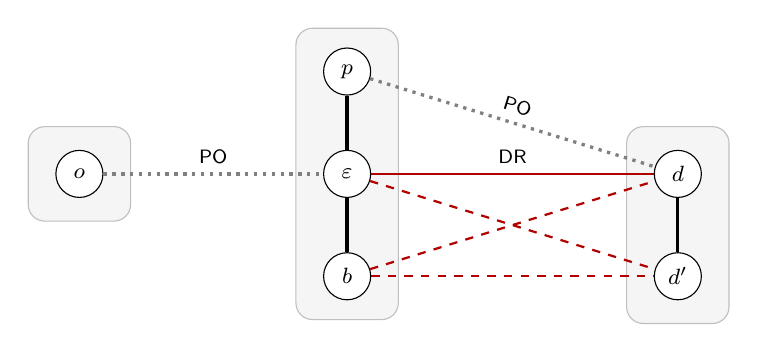
\begin{tikzpicture}[
  occ/.style={circle, draw, fill=white, inner sep=1.2pt, minimum size=17pt, font=\footnotesize},
  treeedge/.style={very thick},
  dr/.style={draw=red!70!black, thick},
  drinh/.style={draw=red!70!black, thick, dashed},
  po/.style={draw=black!50, dotted, very thick},
  comp/.style={draw=black!25, rounded corners=6pt, fill=black!4}]
  \node[comp, minimum width=1.3cm, minimum height=3.7cm] at (0,0) {};
  \node[comp, minimum width=1.3cm, minimum height=2.5cm] at (4.2,-0.65) {};
  \node[comp, minimum width=1.3cm, minimum height=1.2cm] at (-3.4,0) {};
  \node[occ] (p)  at (0,1.3)    {$p$};
  \node[occ] (e)  at (0,0)      {$\varepsilon$};
  \node[occ] (b)  at (0,-1.3)   {$b$};
  \node[occ] (d)  at (4.2,0)    {$d$};
  \node[occ] (dd) at (4.2,-1.3) {$d'$};
  \node[occ] (o)  at (-3.4,0)   {$o$};
  \draw[treeedge] (b) -- (e) -- (p);
  \draw[treeedge] (dd) -- (d);
  \draw[dr] (e) -- node[above, font=\scriptsize] {$\DR$} (d);
  \draw[drinh] (e) -- (dd);
  \draw[drinh] (b) -- (d);
  \draw[drinh] (b) -- (dd);
  \draw[po] (o) -- node[above, font=\scriptsize] {$\PO$} (e);
  \draw[po] (p) -- node[above, sloped, font=\scriptsize] {$\PO$} (d);
\end{tikzpicture}
\caption{Part of a fresh-occurrence unfolding, drawn as a split forest. The
root $\varepsilon$ has four demands, served by $p=(\PP,0)$, $b=(\PPI,1)$,
$d=(\DR,2)$ and $o=(\PO,3)$, and $d$ has a proper part $d'=(\PPI,0)\cdot d$.
The shaded boxes are the connected components of the order, each a tree of
part-of births (thick): $b<\varepsilon<p$ and $d'<d$. Between components
everything is horizontal and read off: $\DR$ at the disjointness birth
$\{\varepsilon,d\}$ (solid) and, by inheritance, between everything below its
two ends (dashed); every other pair, such as $(o,\varepsilon)$ and $(p,d)$, is
$\PO$ (dotted).}
\label{fig:splitforest}
\end{figure}

\paragraph{What the cone scheme keeps, and what it drops.} The two directions
of the proof use the idea differently. The soundness direction \emph{builds} a
split forest: every model the procedure exhibits has that shape, and the two
frame conditions that defeated reuse-based constructions---irreflexivity of the
order, and the order never meeting disjointness---hold because it is a forest
of vertical trees, in which an order edge cannot leave its component and a
disjointness birth opens a new one. The completeness direction does not
\emph{assume} a split forest. It takes an arbitrary model, which need not be
tree-shaped, and uses only the idea's organizing principle, that a point is
characterized by its vertical position: a cone signature is a point's type
together with the types strictly below it. That is also why the transition
conditions push cones along $\PP$ and $\PPI$ and ask nothing structural of
$\PO$. What the earlier routes built in order to \emph{obtain} such a forest
from a given model is gone. There is no appeal to patchwork, because
composition closure follows from the ordered-disjoint axioms
(Theorem~\ref{thm:nf}); no quotient, because no particular model has to be
recovered; and no witness thinning, interface catalogues or width bound,
because completeness needs only that a model's signatures support one another
(Theorem~\ref{thm:complete}).

\paragraph{Why this works on the fragment, and where it stops.} The part of the
split-forest programme that resisted every earlier attempt was control of the
horizontal relations between branches. In the unfolding those relations are
never chosen: disjointness is inherited, and everything else defaults to
overlap. Without $\forall\PO$ no formula can object to that default, so nothing
that crosses between branches needs controlling. With $\forall\PO$ it does---the
unsatisfiable concepts $C_{\mathrm{bad}}$ and $C_{\mathrm{joint}}$ of
\S\ref{ssec:full} are exactly obligations on such cross-branch pairs---and the
interface problem of the original programme returns.

%% ====================================================================
\section{Decision theorems}
\label{sec:main}

\begin{theorem}[Decidability, NNF]\label{thm:main}
For every $\forall\PO$-free NNF concept $C_0$,
\[
  C_0 \text{ is satisfiable} \iff \exists (T,S)\in X_{|\Sigma_0|}:\ C_0\in T .
\]
The right-hand side is a finite computation on lists, so satisfiability of the
fragment is decidable.
\end{theorem}

\begin{proof}
Left to right is Theorem~\ref{thm:complete}. Right to left: $X_{|\Sigma_0|}$ is a
fixed point by Lemma~\ref{lem:gfp}, so Theorem~\ref{thm:sound} applies.
\end{proof}

\subsection{Raw formulas}

Normalization is defined by a single recursion carrying a polarity:
$\mathrm{nnf}^{+}(F)$ is intended to be equivalent to $F$ and
$\mathrm{nnf}^{-}(F)$ to $\neg F$, with $\mathrm{nnf}^{\pm}(\neg F)=
\mathrm{nnf}^{\mp}(F)$ and $\mathrm{nnf}^{-}$ dualizing each constructor.

\begin{theorem}[Decidability, raw formulas]\label{thm:raw}
Both polarities of normalization preserve truth pointwise in every
interpretation, and $\mathrm{Free}^{b}(F)$ implies that $\mathrm{nnf}^{b}(F)$ is
$\forall\PO$-free. Hence satisfiability of formulas $F$ with $\mathrm{Free}^{+}(F)$
is decidable.
\end{theorem}

The polarity condition is forced, not chosen: without it, $\neg\exists\PO.A$
would pass a syntactic ``no $\forall\PO$'' check and normalize to
$\forall\PO.\neg A$. The formal decision procedure for raw input is evaluated by
the Lean kernel on small inputs, which shows that it computes rather than
appealing to excluded middle.

\subsection{Sets and regions}

\begin{corollary}[Set semantics]
Set-satisfiability of $\forall\PO$-free concepts is decidable, by the same
procedure (Theorems~\ref{thm:sets} and~\ref{thm:main}).
\end{corollary}

\begin{corollary}[Regular closed regions]\label{cor:regions}
For each $n>0$, satisfiability of $\forall\PO$-free concepts in substructures of
the RCC5 structure of regular closed regions of $\reals^n$ is decidable, by the
same procedure.
\end{corollary}

\begin{proof}
Lutz and Wolter prove that the logic of general RCC5 structures coincides with
that of substructures of $\reals^n$ with its regular closed
regions~\cite[Thm.~24]{LutzWolter2006}. Directly: the model of
Theorem~\ref{thm:sound} is countable, and every countable general RCC5 structure
is realized by regular closed regions of $\reals^n$~\cite[Thm.~23]{LutzWolter2006}.
\end{proof}

This does \emph{not} extend to the full structure of \emph{all} regular closed
regions of $\reals^n$: a universal restriction there ranges over regions that a
substructure may omit, and the corresponding logics are different; for RCC5
they are undecidable~\cite[Cor.~26]{LutzWolter2006}. The corollary is also
external to the formalization, which proves the set version only.

\subsection{A one-sided test for the full logic}
\label{ssec:full}

Theorem~\ref{thm:complete} never used the fragment.

\begin{corollary}[Sound refutation]\label{cor:unsat}
For every NNF concept $C_0$ and every $n$: if no signature in $X_n$ contains
$C_0$, then $C_0$ is unsatisfiable.
\end{corollary}

The converse fails outside the fragment, and it is instructive to see where.
The concept $\forall\PO.A\sqcap\exists\PO.\neg A$ is refuted in the first round:
its $\PO$ demand needs a target containing both $\neg A$ and, by the $\PO$ row,
$A$ (the kernel checks the same argument for $\exists\PO.\top\sqcap\forall\PO.\bot$,
\code{cpo\_refuted\_at\_one}). But consider
\[
  C_{\mathrm{bad}}=\exists\PPI.(\exists\PP.A)\sqcap\forall\PP.\neg A\sqcap
  \forall\PPI.\neg A\sqcap\neg A\sqcap\forall\PO.\neg A .
\]
The root $x$ and the $A$-point $z$ share a proper part, so
$\rho(x,z)\in\comp(\PPI,\PP)=\{\EQ,\PP,\PPI,\PO\}$, and the four constraints at
the root exclude all four values: $C_{\mathrm{bad}}$ is unsatisfiable. Yet a
family of three signatures---root, part, and $A$-point---supports itself under
$\Prune$, so the test accepts. The obligation lives on the pair $(x,z)$, which no
demand creates and no row of Table~\ref{tab:compat} sees. The same happens with
an explicit overlap demand in
$C_{\mathrm{joint}}=\exists\PP.(\forall\PPI.A\sqcap\forall\PO.A)\sqcap
\exists\PO.\neg A$, whose two witnesses stand in a relation from
$\comp(\PPI,\PO)=\{\PPI,\PO\}$ and either value forces $A$ onto the
$\neg A$-witness. The first of these examples was found by the first cold review
of the formalization and the second by GPT-5.6~Sol's review; we verified both
acceptances on a transcription of the control layer. And the obvious repair,
requiring all witnesses of a signature to be pairwise compatible across $\PO$,
is refuted by the satisfiable
$C_{\mathrm{sat}}=\exists\PP.(A\sqcap\forall\PO.A)\sqcap\exists\PP.\neg A$,
whose two witnesses must be nested, not overlapping. A decision procedure for
the full logic has to reason about the relations \emph{among} contemporaneous
witnesses, not only along the edges that created them.

%% ====================================================================
\section{The formalization}
\label{sec:lean}

\subsection{What is formalized, and how}

The development is written in Lean~4 core, without mathlib, and lives in
\texttt{formal/POFreeLift.lean}, with the forward normal form and the core of
$\eta$ also in \texttt{formal/RCC5NormalForm.lean}~\cite{Artifact}. The file is
cumulative---$45{,}375$ lines, most of them earlier routes
(\S\ref{sec:reflection})---and the cone scheme with its extensions occupies its
last few thousand lines. The development log \texttt{ASSEMBLY\_DESIGN.md},
\S\S267--297, records it step by step.

The encoding is direct. Relations are an inductive type with composition and
converse as functions; concepts are an inductive type in NNF; an interpretation
over a carrier type is a domain predicate, a relation function and a valuation;
satisfaction is structural recursion; and the frame conditions are a structure
over the relation. Satisfiability quantifies over the carrier, so it means
satisfiability in an arbitrary frame. Signatures, the elimination and its
iteration are lists with Boolean tests, so the decision procedure is a program.
Table~\ref{tab:map} maps the results of this paper to declarations.

\begin{table}[t]
\centering
\small
\renewcommand{\arraystretch}{1.2}
\begin{tabular}{@{}L{0.42\textwidth}L{0.52\textwidth}@{}}
\toprule
Result & Lean declarations\\
\midrule
Normal form, Theorem~\ref{thm:nf} & \code{odNet\_frame}, \code{odOfModel},
  \code{odNet\_odOfModel}; \code{toOrderedDisjoint} (\texttt{RCC5NormalForm.lean})\\
Representation, Lemma~\ref{lem:eta}, Theorem~\ref{thm:sets} &
  \code{eta\_sub\_iff}, \code{eta\_disj\_iff}, \code{eta\_inj},
  \code{setRel\_odNet}, \code{satisfiable\_iff\_set}\\
Scheme and elimination, Lemma~\ref{lem:gfp} & \code{sigStatic}, \code{compatB},
  \code{pruneSig\_red}, \code{pruneSig\_mono}, \code{coneScheme\_gfp},
  \code{gfp\_greatest}\\
Completeness, \S\ref{sec:completeness} & \code{dkey\_compat},
  \code{modelSigs\_survives}, \code{modelSigs\_in\_gfp},
  \code{coneScheme\_complete}\\
Unfolding, Lemma~\ref{lem:frame} & \code{Gen}, \code{gOD}, \code{unfInterp\_rcc5},
  \code{unf\_edge\_po}\\
Propagation and truth, Lemma~\ref{lem:truth} & \code{allPP\_gLt},
  \code{allPPI\_gLt}, \code{allDR\_gDisj}, \code{gchild\_serves},
  \code{unf\_truth}\\
Soundness and decision, Theorems~\ref{thm:sound},~\ref{thm:main} &
  \code{coneScheme\_sound}, \code{coneScheme\_correct\_at},
  \code{decidableSat\_cone}\\
Raw formulas, Theorem~\ref{thm:raw} & \code{nnfP\_correct}, \code{pofree\_nnfP},
  \code{decidableFSat}\\
Set semantics & \code{decidableSetSat}\\
Refutation, Corollary~\ref{cor:unsat} & \code{coneScheme\_unsat\_full},
  \code{cpo\_refuted\_at\_one}\\
\bottomrule
\end{tabular}
\caption{Results and their Lean declarations, all in
\texttt{formal/POFreeLift.lean} unless marked.}
\label{tab:map}
\end{table}

The capstones have these types:
\begin{quote}\footnotesize
\code{decidableSat\_cone (C0 : Concept) (hpo : POFree C0) : Decidable (Satisfiable C0)}\\
\code{decidableFSat (F : Formula) (h : FPOFree true F) : Decidable (FSatisfiable F)}\\
\code{satisfiable\_iff\_set (C0 : Concept) : Satisfiable C0 <-> SetSatisfiable C0}
\end{quote}

\subsection{Checking it}

The file builds with Lean~4.33.1 in under a minute
(\texttt{cd formal \&\& lean POFreeLift.lean}), with no errors, warnings or
\texttt{sorry}; earlier builds used 4.32.0. The source contains no
\texttt{axiom} declaration, no \texttt{native\_decide}, and no \texttt{unsafe},
\texttt{partial} or \texttt{implemented\_by}. The capstones depend on the axioms
\texttt{propext}, \texttt{Classical.choice} and \texttt{Quot.sound}. Classical
reasoning enters where arbitrary interpretations are handled---the type of a
point is defined by a classical case distinction on satisfaction---and in the
induced labelling of an ordered-disjoint structure, which decides order and
disjointness classically; the decision procedure itself computes on lists, and
the kernel evaluates it on small inputs. The polarity lemma \code{pofree\_nnfP}
and the unsatisfiability of $\exists\PO.\top\sqcap\forall\PO.\bot$
(\code{cpo\_unsat}) use no axioms at all. The repository does not yet pin a toolchain file or provide a minimal
build target containing only the dependency closure of the capstones; both are
release engineering, not premises of the theorem.

\subsection{What machine checking does and does not settle}

The kernel guarantees that the theorems follow from the definitions. It cannot
guarantee that the definitions mean what this paper says they mean, and three
things in the paper are not formal theorems: the absence of finite models in
Example~\ref{ex:inf} (only satisfiability of $C_\infty$ is formalized), the
complexity bound of \S\ref{sec:complexity}, and the transfer to regular closed
regions in Corollary~\ref{cor:regions}, which cites Lutz and Wolter.
Definitional adequacy is what the reviews below were aimed at, and the
equivalence with set semantics was proved partly so that it need not rest on
anyone's reading of the frame conditions.

\subsection{Reviews}
\label{ssec:reviews}

The formalization was reviewed by three fresh model sessions with no access to
its development history, each targeting a different part, and later audited at
source level by a fourth~\cite{GPT56SolReview}.
\begin{itemize}
  \item The first built the file under two Lean versions, re-derived the
    composition table from set semantics, compared a transcription of the
    control layer with exhaustive search over small models on $4{,}000$ random
    fragment concepts, and
    found two comments that misstated where the fragment hypothesis is used and
    an enumeration of types that was larger than necessary by an exponential.
  \item The second attacked completeness, ran the elimination on $6{,}268$
    concepts against exhaustive model search without rejecting a satisfiable
    one, and found that the $\PO$ row of Table~\ref{tab:compat} had been
    omitted. Restoring it left the fragment result untouched---the row is
    vacuous there---and made the refutation test of \S\ref{ssec:full} strictly
    stronger.
  \item The third attacked soundness, running the unfolding on labels taken from
    actual greatest fixed points: $2{,}157$ accepted concepts, $6{,}464$
    unfoldings and $10{,}066$ occurrences, with no violation of the frame
    conditions or of the truth lemma. Its findings concerned the project's own
    test scripts and prose.
  \item The fourth, by GPT-5.6~Sol, located every capstone of the decision
    chain in the source and found no hidden hypothesis; its findings concerned
    how the companion overview described the result.
\end{itemize}
No review found a counterexample to the theorem.

%% ====================================================================
\section{Complexity and practicality}
\label{sec:complexity}

With $m=|\cl(C_0)|$ there are at most $2^m$ candidate types and
$|\Sigma_0|\le 2^m\cdot 2^{2^m}$ signatures. The procedure performs at most
$|\Sigma_0|$ rounds, and a round compares every signature and demand with every
candidate target, each comparison being polynomial in $m$ and $2^m$. The running
time is therefore bounded by $2^{2^{O(m)}}$, doubly exponential in the size of
$C_0$. This bound is not formalized, and no lower bound beyond what the fragment
inherits is established here.

The bound describes the literal procedure, and the literal procedure is
impractical: it materializes the power set of the type space, and in the project's
measurements it can be run only on concepts with a handful of subconcepts. A
symbolic implementation---antichains of spectra, decision diagrams, or a SAT
encoding of the elimination---is the obvious next step, but it would need its
own correctness proof. Merging spectra that agree on the currently relevant
bodies is exactly the kind of identification that this construction avoids,
and it could reintroduce the problems it removed.

%% ====================================================================
\section{Why reuse failed, and what \texorpdfstring{$\forall\PO$}{forall-PO} breaks}
\label{sec:reflection}

The cone scheme was not the first attempt to certify this fragment. The
fragment was isolated in April 2026 by a two-tier quotient
construction~\cite{TwoTierQuotient} and re-derived twice by other
arguments~\cite{Overview}, but formalizing it on those lines required a finite
set of nodes, reused by blocking, with witnesses borrowed from one node for
another. Four successive disciplines for that reuse were refuted by exact finite
countermodels: a per-edge safety test (two individually safe fallback edges
formed a four-cycle), a class representative chosen by type (it dragged one
member's disjointness witness under another member), a key computed from an
occurrence's downward cone (the obstruction was horizontal, so the key could not
separate the occurrences), and repeat-free selection.

The failures had one cause. Reusing a node imposes a global condition on the
object being built---the order induced by the reused edges must be acyclic, and
the relations those edges force must be jointly realizable---and each discipline
was a local test, on an edge, a node or a type. Blocking in the usual sense is
the same local test: two occurrences with equal types, so let one stand for the
other. Equal types cannot show whether the substitution closes a cycle in the
order or places a disjointness witness below a node it must be disjoint from.
The cone scheme does not test more carefully; it removes the obligation. Nothing
is reused, so the order is irreflexive because heights increase, and
disjointness never meets the order because a $\DR$ birth changes the vertical
base. GPT-5.6~Sol proposed this change of architecture when asked for an
alternative to repairing the reuse route~\cite{GPT56Sol}.

What $\forall\PO$ breaks is then easy to name. The unfolding labels every
residual pair $\PO$, and without $\forall\PO$ no residual pair is constrained.
With $\forall\PO$, the relations among contemporaneous witnesses matter, as
$C_{\mathrm{bad}}$ and $C_{\mathrm{joint}}$ show, and a construction for the
full logic has to choose them jointly. Three directions look promising: control
states that carry a complete RCC5 matrix among representatives of
simultaneously live demands, whose completeness is where a bound on joint width
would have to be proved; regular or automatic presentations of models; and a
recasting of ordered-disjoint structures as a single strict order on two copies
of the domain, which brings the problem close to two-variable logic with one
transitive relation~\cite{SzwastTendera2013} but adds an involution that keeps
the copies synchronized. The last two were suggested by GPT-5.6~Sol's
review~\cite{GPT56SolReview}. Any candidate must reject $C_{\mathrm{bad}}$ and
accept $C_{\mathrm{sat}}$.

%% ====================================================================
\section{Related work}
\label{sec:related}

\paragraph{Spatial description logics and modal logics of regions.} Cohn
proposed modal and non-modal qualitative spatial logics~\cite{Cohn1993}. Wessel
introduced the $\mathcal{ALCI}_{\mathrm{RCC}}$ family, settled its coarser members,
and left the RCC5 and RCC8 cases open~\cite{Wessel2003}; the same report
canvassed restricted fragments that regain the finite model property, which the
present fragment does not. Lutz and Wolter~\cite{LutzWolter2006} introduced modal
logics of topological relations. For RCC5 they proved the representation and
logic-equivalence results used above (Theorems~23 and~24), recursive
enumerability of the logics of general structures (Theorem~28), and
undecidability for classes of structures closed under certain suprema
(Theorem~25); they left the general case open. They also remarked that dropping
$\PO$ has been argued to leave a useful formalism for geographic applications,
pointing to work of Shapirovsky and Shehtman on a single inclusion
modality~\cite{ShapirovskyShehtman2005}; that remark concerns usefulness and
carries no decidability argument. Our fragment keeps $\PO$ and $\exists\PO$ and
removes only the universal. So far as we can determine, no decidability result
for a $\PO$-restricted RCC5 language has been published.

\paragraph{Constraint reasoning.} Consistency of finite networks of RCC
relations is the subject of qualitative constraint reasoning; Renz and Nebel
analysed its complexity for RCC8~\cite{RenzNebel1999}. For atomic RCC5 networks
with strong equality, path consistency implies consistency, which is
Theorem~\ref{thm:nf}(b) together with Lemma~\ref{lem:eta} read for finite
structures. Concept satisfiability adds
unary predicates, arbitrary nesting and infinite models, so constraint
consistency is an ingredient here, not a decision procedure.

\paragraph{Concrete domains.} Description logics with concrete
domains~\cite{LutzMilicic2007,BaaderRydval2020} attach spatial values to abstract
objects through features. The closest of them, $\mathcal{ALCRP}(D)$, forms roles
from concrete predicates and so quantifies over spatial relations; it is
undecidable in general and decidable under syntactic
restrictions~\cite{HaarslevLutzMoeller1999}. It stays two-sorted: equal extensions
need not be equal objects, and objects without the feature stand in no spatial
relation.

\paragraph{Event structures and two-variable logic.} The ordered-disjoint normal
form matches the order and conflict skeleton of prime event
structures~\cite{NielsenPlotkinWinskel1981}. Two-variable first-order logic with
one transitive relation is decidable~\cite{SzwastTendera2013}; whether the
synchronized two-copy encoding of \S\ref{sec:reflection} can use that is open.

\paragraph{Formalization.} The proof is checked in Lean~4~\cite{Lean4}. Its
cumulative development, including the refuted routes, is public.

%% ====================================================================
\section{Provenance and contributions}
\label{sec:provenance}

The result was produced by a long human--model collaboration, and the record of
who did what is public~\cite{ConversationLog}. We state it here for this result
specifically.

\begin{itemize}
  \item \textbf{Michael Wessel} posed the problem in 2002/2003, supplied the
    split-forest representation---vertical nesting plus horizontal
    completion---whose shape the unfolding builds (\S\ref{ssec:splitforest}),
    and the kernel idea from which
    the fragment was first isolated. He directed the work throughout, stopped
    the repair of the reuse architecture when it began to cycle, asked a fresh
    model for an alternative, and decided on the split into two papers.
  \item \textbf{Claude} (Anthropic) built the two-tier quotient construction
    that first isolated the fragment (April 2026). Claude~Fable~5 formalized the
    normal form and the core of $\eta$ (July 2026); Claude~Opus~4.8 formalized
    the logic layer on which the truth lemma rests (July 2026); Claude~Opus~5
    formalized the cone scheme, the normalization of raw formulas and the
    equivalence with set semantics (August 2026), and wrote this paper.
  \item \textbf{GPT-5.4~Pro} (OpenAI) reviewed the two-tier construction and
    exposed the overlap gap that located the fragment's boundary.
    \textbf{GPT-5.5} re-derived the fragment independently in a cold attack on
    the open problem, and its regular-cover analysis produced the
    ordered-disjoint normal form. \textbf{GPT-5.6~Pro} gave the canonical set
    representation $\eta$~\cite{GPT56TechNote}.
  \item \textbf{GPT-5.6~Sol} (OpenAI) designed the cone scheme: retire node
    reuse, keep the finite scheme only as a control graph, and unfold every
    non-$\EQ$ demand to a fresh occurrence~\cite{GPT56Sol}. Later, in a cold
    review of the overview, it recommended separating this result into a
    focused paper and wrote a draft of one~\cite{GPT56SolReview}.
  \item \textbf{Three fresh model sessions} reviewed the formalization cold
    (\S\ref{ssec:reviews}); their findings are incorporated.
\end{itemize}

\paragraph{How this text relates to the draft.} GPT-5.6~Sol's draft is archived
unmodified with its review~\cite{GPT56SolReview}. The recommendation to write a
focused paper, and its outline---normal form, scheme, completeness, soundness,
decision theorems, formalization, open problem---are that review's. The text is
not: it was written anew from the Lean sources, and it departs from the draft
where our own checks led elsewhere. It credits Lutz and Wolter's Theorem~23 for
the set representation, which the draft listed among its contributions; it marks
which statements are cited or argued in prose rather than checked by the kernel;
it adds the boundary examples of \S\ref{ssec:full}, with their status verified
against the control layer; and it records provenance in full.

\paragraph{Artifacts.} The repository is
\url{https://github.com/lambdamikel/alcircc5}. The formal files are
\texttt{formal/POFreeLift.lean} and \texttt{formal/RCC5NormalForm.lean}. This
paper, the overview, and the Lean artifact are frozen at git tag
\texttt{release-2026-09-14}; its Lean sources differ from those at the earlier
tag \texttt{certified-fragment-2026-08-29} only in the spelling of comments.
Cite the tag or its commit hash rather than the \texttt{master} branch. The review and draft are in
\texttt{papers/gpt-5.6-latest-overview-paper-review-and-recommendation/}, and
the overview is \texttt{papers/overview\_arxiv.tex}.

\bigskip
\noindent\textbf{AI disclosure.} The mathematics, the formalization and this
text were produced by the AI systems named above under the direction of the
human author, who is responsible for the paper. The results are
machine-checked where stated and have not yet been reviewed by human experts in
description logic or qualitative spatial reasoning; we would welcome that
review.

%% ====================================================================
\begin{thebibliography}{99}

\bibitem{BaaderRydval2020}
F.\ Baader and M.\ Rydval.
\newblock Description logics with concrete domains and general concept
  inclusions revisited.
\newblock In \emph{Proc.\ IJCAR}, volume 12166 of LNCS, pages 413--431.
  Springer, 2020.

\bibitem{Cohn1993}
A.\,G.\ Cohn.
\newblock Modal and non modal qualitative spatial logics.
\newblock In F.\,D.\ Anger, H.\,W.\ Guesgen, and J.\ van Benthem, editors,
  \emph{Proceedings of the Workshop on Spatial and Temporal Reasoning},
  IJCAI, 1993.

\bibitem{Lean4}
L.\ de Moura and S.\ Ullrich.
\newblock The Lean~4 theorem prover and programming language.
\newblock In \emph{Automated Deduction -- CADE 28}, volume 12699 of LNCS,
  pages 625--635. Springer, 2021.

\bibitem{HaarslevLutzMoeller1999}
V.\ Haarslev, C.\ Lutz, and R.\ M\"oller.
\newblock A description logic with concrete domains and a role-forming
  predicate operator.
\newblock \emph{Journal of Logic and Computation}, 9(3):351--384, 1999.

\bibitem{LutzMilicic2007}
C.\ Lutz and M.\ Mili\v{c}i\'{c}.
\newblock A tableau algorithm for description logics with concrete domains and
  general TBoxes.
\newblock \emph{Journal of Automated Reasoning}, 38:227--259, 2007.

\bibitem{LutzWolter2006}
C.\ Lutz and F.\ Wolter.
\newblock Modal logics of topological relations.
\newblock \emph{Logical Methods in Computer Science}, 2(2:5):1--41, 2006.
\newblock \url{https://doi.org/10.2168/LMCS-2(2:5)2006}

\bibitem{NielsenPlotkinWinskel1981}
M.\ Nielsen, G.\ Plotkin, and G.\ Winskel.
\newblock Petri nets, event structures and domains, part~I.
\newblock \emph{Theoretical Computer Science}, 13(1):85--108, 1981.

\bibitem{RenzNebel1999}
J.\ Renz and B.\ Nebel.
\newblock On the complexity of qualitative spatial reasoning:
  A maximal tractable fragment of the Region Connection Calculus.
\newblock \emph{Artificial Intelligence}, 108(1--2):69--123, 1999.

\bibitem{ShapirovskyShehtman2005}
I.\ Shapirovsky and V.\ Shehtman.
\newblock Modal logics of regions and Minkowski spacetime.
\newblock \emph{Journal of Logic and Computation}, 15(4):559--574, 2005.

\bibitem{SzwastTendera2013}
W.\ Szwast and L.\ Tendera.
\newblock $\mathrm{FO}^2$ with one transitive relation is decidable.
\newblock In \emph{Proc.\ STACS 2013}, LIPIcs~20, pages 317--328, 2013.

\bibitem{Wessel2003}
M.\ Wessel.
\newblock Qualitative spatial reasoning with the $\ALCIRCC{}$ family ---
  first results and unanswered questions.
\newblock Technical Report FBI-HH-M-324/03, Fachbereich Informatik,
  Universit\"at Hamburg, 2002/2003.
\newblock \url{https://github.com/lambdamikel/alcircc5/blob/master/papers/report7.pdf}

%% --- project documents ---

\bibitem{Overview}
M.\ Wessel (with AI assistants).
\newblock Can agentic AI settle a 20-year-old description logic problem? On the
  decidability of $\ALCIRCC{5}$: a machine-checked decidable fragment and a map
  of what remains open.
\newblock Overview paper, September 2026.
\newblock \url{https://github.com/lambdamikel/alcircc5/blob/master/papers/overview_arxiv.pdf}

\bibitem{TwoTierQuotient}
Claude (Anthropic), prompted by M.\ Wessel.
\newblock A two-tier quotient construction for the PO-coherent fragment of
  $\ALCIRCC{5}$.
\newblock Technical report, April 2026.
\newblock \url{https://github.com/lambdamikel/alcircc5/blob/master/papers/two_tier_quotient_ALCIRCC5.pdf}

\bibitem{GPT56TechNote}
GPT-5.6 Pro (OpenAI), prompted by M.\ Wessel.
\newblock A canonical set representation for $\ALCIRCC{5}$: the converse of the
  ordered-disjoint RCC5 normal form (technical note).
\newblock Technical report, July 2026.
\newblock File
  \texttt{papers/final\_paper\_gpt\_5.6\_review/ALCI\_RCC5\_F6\_technical\_note.pdf}.

\bibitem{GPT56Sol}
GPT-5.6 Sol (OpenAI), prompted by M.\ Wessel.
\newblock A Lean certification plan for the $\forall\PO$-free fragment of
  $\ALCIRCC{5}$: the cone-scheme blueprint.
\newblock Technical report, August 2026.
\newblock Directory \texttt{papers/cone\_scheme\_plan/}.

\bibitem{GPT56SolReview}
GPT-5.6 Sol (OpenAI), prompted by M.\ Wessel.
\newblock Cold review of the current $\ALCIRCC{5}$ development, with a draft
  focused paper on the $\forall\PO$-free fragment.
\newblock Review report, 9~September 2026, of commit \texttt{795b270}.
\newblock Directory
  \texttt{papers/gpt-5.6-latest-overview-paper-review-and-recommendation/}.

\bibitem{Artifact}
M.\ Wessel (with AI assistants).
\newblock $\ALCIRCC{5}$ project repository: Lean formalization, verification
  probes, papers and review record.
\newblock \url{https://github.com/lambdamikel/alcircc5}

\bibitem{ConversationLog}
M.\ Wessel (with AI assistants).
\newblock \texttt{CONVERSATION.md}: the project conversation log, for auditable
  attribution.
\newblock \url{https://github.com/lambdamikel/alcircc5/blob/master/CONVERSATION.md}

\end{thebibliography}

\end{document}
